\chapter{Волновые функции осциллятора, спин 1/2 и перестановка частиц}

\section{Осцилляторы повсюду}

Любая система с устойчивым равновесием может колебаться, если ее вывести из этого равновесия. У нее может быть одна частота или много. У струны скрипки, например, есть основная мода и высшие гармоники. Если ее щипнуть, возбуждается некоторая комбинация этих мод.

Более важные для нас примеры здесь — поля. Равновесная конфигурация электромагнитного поля — это вакуум: нет ни электрического поля, ни магнитного поля, ни электромагнитных колебаний. Если ввести излучение в полость или волновод, поле может колебаться в своих разрешенных модах, каждая со своей собственной частотой. В квантовой теории эти моды описывают совокупности фотонов.

Та же идея применима к кристаллу. Представлять каждый атом как независимый осциллятор вводит в заблуждение. Атомы действуют друг на друга силами, так что смещение одного атома влияет на его соседей, и через кристалл проходит волна. Нормальные моды этого связанного движения являются гармоническими осцилляторами, а их кванты называются фононами. Фотоны и фононы — разные физические объекты, но и те и другие приводят к одной и той же алгебре осциллятора.

\section{Алгебра осциллятора}

При обсуждении осциллятора положим массу и приведенную постоянную Планка равными 1:
\[
m=1,\qquad \hbar=1.
\]
Гамильтониан имеет вид
\begin{equation}
H=\frac{p^{2}}{2}+\frac{\omega^{2}x^{2}}{2}.
\end{equation}
Параметр \(\omega\) задает кривизну потенциала и одновременно является частотой колебаний.

Введем операторы повышения и понижения:
\begin{equation}
A_{\pm}=\frac{p\pm i\omega x}{\sqrt{2\omega}}.
\end{equation}
Нормировка выбрана так, что
\begin{equation}
[A_{-},A_{+}]=1.
\end{equation}
Оператор числа имеет вид
\begin{equation}
N=A_{+}A_{-}.
\end{equation}
Вместе эти уравнения означают, что \(A_{+}\) увеличивает собственное значение \(N\) на единицу, а \(A_{-}\) уменьшает его на единицу. Получающийся спектр таков:
\begin{equation}
n=0,1,2,3,\ldots .
\end{equation}

Произведение двух лестничных операторов также выявляет квантовую поправку к классической энергии:
\begin{align}
N
&=\frac{1}{2\omega}(p+i\omega x)(p-i\omega x)\\
&=\frac{1}{2\omega}\left(p^{2}+\omega^{2}x^{2}
 +i\omega[x,p]\right)\\
&=\frac{1}{2\omega}\left(p^{2}+\omega^{2}x^{2}-\omega\right),
\end{align}
где \([x,p]=i\). Следовательно,
\begin{equation}
H=\omega\left(N+\frac12\right).
\end{equation}
Если аддитивная константа для задачи несущественна, удобно использовать сдвинутый гамильтониан
\begin{equation}
H_{\mathrm{shifted}}=H-\frac{\omega}{2}=\omega N.
\end{equation}
Член \(\omega/2\) — это энергия нулевых колебаний осциллятора, то есть энергия основного состояния. Для моды поля аналогичный член называется энергией вакуума. Он отражает принцип неопределенности: ни одно состояние не может иметь одновременно \(x\) и \(p\), точно равные нулю, так что два положительных квадратичных члена в \(H\) не могут оба иметь нулевое среднее значение.

\begin{classroomqa}
\lecturetimestamp{00:09:46}
\audiencequestion{Почему нуль входит в спектр оператора числа?}
\lecturerresponse{Это можно явно показать, построив волновую функцию основного состояния. Это построение выявит состояние с \(N=0\).}
\end{classroomqa}

Чтобы начать это построение, заменим векторы состояния волновыми функциями координаты. Собственные состояния энергии принимают вид
\[
\psi_{0}(x),\ \psi_{1}(x),\ \psi_{2}(x),\ldots,
\]
а основные операторы действуют как
\begin{equation}
X\longmapsto x,\qquad
P\longmapsto -i\frac{d}{dx}.
\end{equation}
Если восстановить \(\hbar\), вторая замена примет вид
\(P\mapsto-i\hbar\,d/dx\).

Прежде чем решать для \(\psi_{0}\), на этот вопрос есть более быстрый абстрактный ответ. На дискретной лестнице нормируемых собственных состояний осциллятора \(N=A_{+}A_{-}\) неотрицателен, поэтому многократное понижение шагами по единице не может продолжаться бесконечно. В нижнем конце---чью нормируемую волновую функцию мы построим ниже---должно существовать состояние, обозначаемое \(\lvert0\rangle\), для которого
\begin{equation}
A_{-}\lvert0\rangle=\mathbf 0.
\end{equation}
Иначе \(A_{-}\lvert0\rangle\) было бы еще одним состоянием на одну ступень ниже. Отсюда сразу следует, что
\begin{equation}
N\lvert0\rangle
=A_{+}A_{-}\lvert0\rangle
=\mathbf 0
=0\,\lvert0\rangle.
\end{equation}
Таким образом, нижнее состояние имеет нулевое собственное значение оператора числа.

\begin{classroomqa}
\lecturetimestamp{00:14:57}
\audiencequestion{Если собственное значение равно нулю, не должен ли правый член содержать нулевой собственный вектор?}
\lecturerresponse{Кет \(\lvert0\rangle\) — это нормированный ненулевой вектор с меткой нуль. В \(N\lvert0\rangle=0\,\lvert0\rangle\) правая часть — нулевой вектор. Кет основного состояния и нулевой вектор — разные объекты.}
\end{classroomqa}

\section{Уравнение Schr\"odinger и физические решения}

Теперь вернемся к координатному представлению. Стационарное уравнение Schr\"odinger имеет вид
\begin{equation}
\left[
-\frac12\frac{d^{2}}{dx^{2}}
+\frac12\omega^{2}x^{2}
\right]\psi(x)=E\psi(x).
\end{equation}
Как дифференциальное уравнение второго порядка, оно имеет формальные решения при произвольных значениях \(E\). Большинство этих формальных решений не являются физическими состояниями осциллятора. При больших \(\lvert x\rvert\) они растут экспоненциально, так что их норма расходится.

Для связанного состояния волновая функция должна быть квадратично интегрируемой:
\begin{equation}
\int_{-\infty}^{\infty}\psi^{*}(x)\psi(x)\,dx<\infty.
\end{equation}
Тогда ее можно нормировать так, чтобы интеграл был равен единице. Только специальные значения энергии дают такие решения. Координатные и импульсные состояния на бесконечной прямой в этом отношении составляют исключение, но экспоненциально растущие решения осциллятора просто исключаются из пространства состояний.

\section{Гауссово основное состояние}

Уравнение второго порядка можно решить, но алгебра лестничных операторов дает более простое уравнение первого порядка:
\begin{equation}
A_{-}\psi_{0}(x)=0.
\end{equation}
Общий множитель в \(A_{-}\) несущественен, когда правая часть равна нулю, поэтому это равносильно
\begin{equation}
(p-i\omega x)\psi_{0}(x)=0.
\end{equation}
Используя \(p=-i\,d/dx\), получаем
\begin{equation}
\left(\frac{d}{dx}+\omega x\right)\psi_{0}(x)=0.
\end{equation}

\begin{classroomqa}
\lecturetimestamp{00:22:32}
\audiencequestion{Можно ли было бы решить это разделением переменных?}
\lecturerresponse{Здесь есть только одна независимая переменная, так что двух переменных для разделения нет. В записи \(\psi_{0}'/\psi_{0}=-\omega x\) это уравнение имеет вид логарифмической производной. Это подсказывает записать волновую функцию в экспоненциальной форме.}
\end{classroomqa}

Удобно искать решение в виде
\begin{equation}
\psi_{0}(x)=e^{f(x)}.
\end{equation}
Тогда
\[
\psi_{0}'(x)=f'(x)e^{f(x)},
\]
и общий экспоненциальный множитель сокращается. Уравнение сводится к
\begin{equation}
\frac{df}{dx}+\omega x=0.
\end{equation}

\begin{classroomqa}
\lecturetimestamp{00:26:28}
\audiencequestion{Не должен ли в \(f(x)\) стоять знак минус?}
\lecturerresponse{Да. Поскольку \(df/dx=-\omega x\), интегрирование дает отрицательный квадратичный член.}
\end{classroomqa}

Следовательно,
\begin{equation}
f(x)=-\frac12\omega x^{2}+C,
\end{equation}
и
\begin{equation}
\psi_{0}(x)\propto e^{-\omega x^{2}/2}.
\end{equation}
Мультипликативная нормировочная константа оставлена неопределенной. Важна гауссова форма: функция гладкая, сосредоточена вблизи начала координат и быстро убывает при больших \(\lvert x\rvert\). Она очевидным образом квадратично интегрируема.

Нет необходимости подставлять ответ обратно в уравнение второго порядка, чтобы узнать его энергию. Алгебра уже дает
\begin{equation}
E_{0}=\frac{\omega}{2}.
\end{equation}

\section{Возбужденные состояния, узлы и классическое движение}

Первое возбужденное состояние получается действием оператора повышения на основное состояние:
\begin{equation}
\psi_{1}(x)\propto A_{+}\psi_{0}(x)
\propto(p+i\omega x)e^{-\omega x^{2}/2}.
\end{equation}
Из уравнения для основного состояния следует
\[
p\psi_{0}=i\omega x\,\psi_{0}.
\]
Смена знака в лестничном операторе превращает сокращение в сложение:
\begin{equation}
(p+i\omega x)\psi_{0}
=2i\omega x\,\psi_{0}.
\end{equation}
С точностью до общего множителя,
\begin{equation}
\psi_{1}(x)\propto x\,e^{-\omega x^{2}/2}.
\end{equation}

Эта волновая функция нечетна:
\begin{equation}
\psi_{1}(-x)=-\psi_{1}(x).
\end{equation}
Ее плотность вероятности четна, но в начале координат у нее есть узел,
\begin{equation}
\lvert\psi_{1}(0)\rvert^{2}=0.
\end{equation}
Следовательно, плотность вероятности первого возбужденного состояния имеет узел при \(x=0\).

Многократное действие \(A_{+}\) дает многочлены все более высокой степени, умножающие ту же гауссову оболочку.\footnote{В лекции указаны многочленные множители более высокой степени, дополнительный узел на каждом шаге и чередование четности в промежутке от \(00{:}34{:}25\) до \(00{:}35{:}49\). Вид произведения гауссиана на многочлен подтверждается также в книге Leonard Susskind и Art Friedman, \emph{Quantum Mechanics: The Theoretical Minimum} (2014), при обсуждении собственных функций осциллятора.} С точностью до нормировки,
\begin{equation}
\psi_{n}(x)=P_{n}(x)e^{-\omega x^{2}/2}.
\end{equation}
Четность чередуется между четной и нечетной, и каждый шаг добавляет узел. С ростом \(n\) волновая функция простирается дальше от начала координат и приобретает более быстрые осцилляции.

Эти две особенности имеют прямой физический смысл. То, что волновая функция заметна дальше от начала координат, соответствует большей потенциальной энергии, потому что потенциал растет как \(x^{2}\). Быстрые осцилляции в координатном пространстве указывают на больший импульс. Сильно возбужденный осциллятор с большей вероятностью удаляется дальше от центра; когда он проходит через центральную область, он несет больший импульс, и там его волновая функция осциллирует быстрее.

\begin{classroomqa}
\lecturetimestamp{00:37:18}
\audiencequestion{Разве гармонический осциллятор не приближается к классическому поведению, когда \(n\) становится большим?}
\lecturerresponse{Классическое движение не представляется одним стационарным собственным состоянием энергии. Оно возникает в волновом пакете, содержащем много энергетических уровней. Сдвинутый гауссиан, например, эволюционирует туда и обратно как классический осциллятор, а относительная неопределенность становится меньше по мере того, как размах колебаний растет.}
\end{classroomqa}

Возьмем гауссиан основного состояния и сместим его от начала координат. Сдвинутый пакет больше не является собственным состоянием энергии; он представляет собой суперпозицию многих таких состояний. Согласно зависящему от времени уравнению Schr\"odinger его компоненты приобретают разные фазы. Пакет колеблется от одной стороны потенциала к другой, приобретая быстрые изменения фазы вблизи центра и снова становясь гладким вблизи точки поворота. Чем больше размах по сравнению с шириной пакета, тем ближе движение к классическому.

\begin{classroomqa}
\lecturetimestamp{00:39:29}
\audiencequestion{Должна ли волновая функция второго возбужденного состояния проходить через нуль в начале координат?}
\lecturerresponse{Нет. Ее многочленный множитель — не просто \(x^{2}\); он также содержит постоянный член, так что волновая функция не обязана обращаться в нуль при \(x=0\).}
\end{classroomqa}

Аргумент с лестничными операторами также предполагает, что \(A_{+}\) и \(A_{-}\) являются эрмитово-сопряжёнными друг другу на области определения осциллятора, состоящей из квадратично интегрируемых функций, с граничным поведением, необходимым для соотношения сопряжённости. Формальные решения, растущие экспоненциально, этой области не принадлежат.

\begin{classroomqa}
\lecturetimestamp{00:40:45}
\audiencequestion{Существует ли общий способ распознать, когда гамильтониан может быть решён этими алгебраическими методами?}
\lecturerresponse{Такого общего правила нет. Точно решаемые примеры редки. Гармонический осциллятор и идеальный нерелятивистский атом водорода — удачные случаи, в которых алгебраические методы работают.}
\end{classroomqa}

\section{Спин 1/2 как момент импульса}

Спин — это момент импульса, которым частица обладает независимо от орбитального движения своего центра масс. Покоящаяся частица не имеет орбитального момента импульса \(\mathbf R\times\mathbf P\), но всё же может иметь спин. Можно пытаться представить себе крошечный вращающийся объект или рассматривать спин как внутреннее квантовое свойство. Решающим является математическое утверждение: его компоненты преобразуются при пространственных вращениях и удовлетворяют коммутационным соотношениям для момента импульса.

Начиная с этого места, снова восстановим \(\hbar\). Компоненты момента импульса удовлетворяют
\begin{equation}
[L_{z},L_{x}]=i\hbar L_{y},
\end{equation}
а два других соотношения получаются циклической перестановкой. Безразмерные матрицы Паули имеют вид
\begin{equation}
\begin{aligned}
\sigma_{z}&=
\begin{pmatrix}
1&0\\
0&-1
\end{pmatrix},\\[0.4em]
\sigma_{x}&=
\begin{pmatrix}
0&1\\
1&0
\end{pmatrix},\\[0.4em]
\sigma_{y}&=
\begin{pmatrix}
0&-i\\
i&0
\end{pmatrix}.
\end{aligned}
\end{equation}
В этом базисе \(\sigma_{z}\) диагональна. Её собственные значения равны \(+1\) и
\(-1\).

\begin{classroomqa}
\lecturetimestamp{00:47:35}
\audiencequestion{Есть ли знак минус в \(\sigma_x\)?}
\lecturerresponse{Нет. Оба внедиагональных элемента \(\sigma_x\) положительны.}
\end{classroomqa}

Вычисление на доске в \(00{:}49{:}35\) начинает покомпонентное
умножение матриц. Доведение произведений до конца даёт
\begin{align}
\sigma_{z}\sigma_{x}
&=
\begin{pmatrix}
0&1\\
-1&0
\end{pmatrix}
=i\sigma_{y},\\
\sigma_{x}\sigma_{z}
&=
\begin{pmatrix}
0&-1\\
1&0
\end{pmatrix}
=-i\sigma_{y}.
\end{align}
Следовательно,
\begin{equation}
[\sigma_{z},\sigma_{x}]=2i\sigma_{y}.
\end{equation}
Лишний множитель 2 устраняется, если определить физические операторы спина как\footnote{Вычисление на доске опускает \(\hbar\). Здесь он восстановлен, так что \(S_i\) имеет размерность момента импульса.}
\begin{equation}
S_{i}=\frac{\hbar}{2}\sigma_{i}.
\end{equation}
Тогда
\begin{equation}
[S_{z},S_{x}]=i\hbar S_{y},
\end{equation}
и аналогично для циклических перестановок. Следовательно, половины матриц Паули, с восстановленным множителем \(\hbar\), образуют систему момента импульса.

Положив \(\hbar=1\), получаем вид, показанный ниже.\footnote{Исходный кадр — \texttt{lecture\_04\_frame\_02.png}.}
\begin{figure}[htbp]
\centering
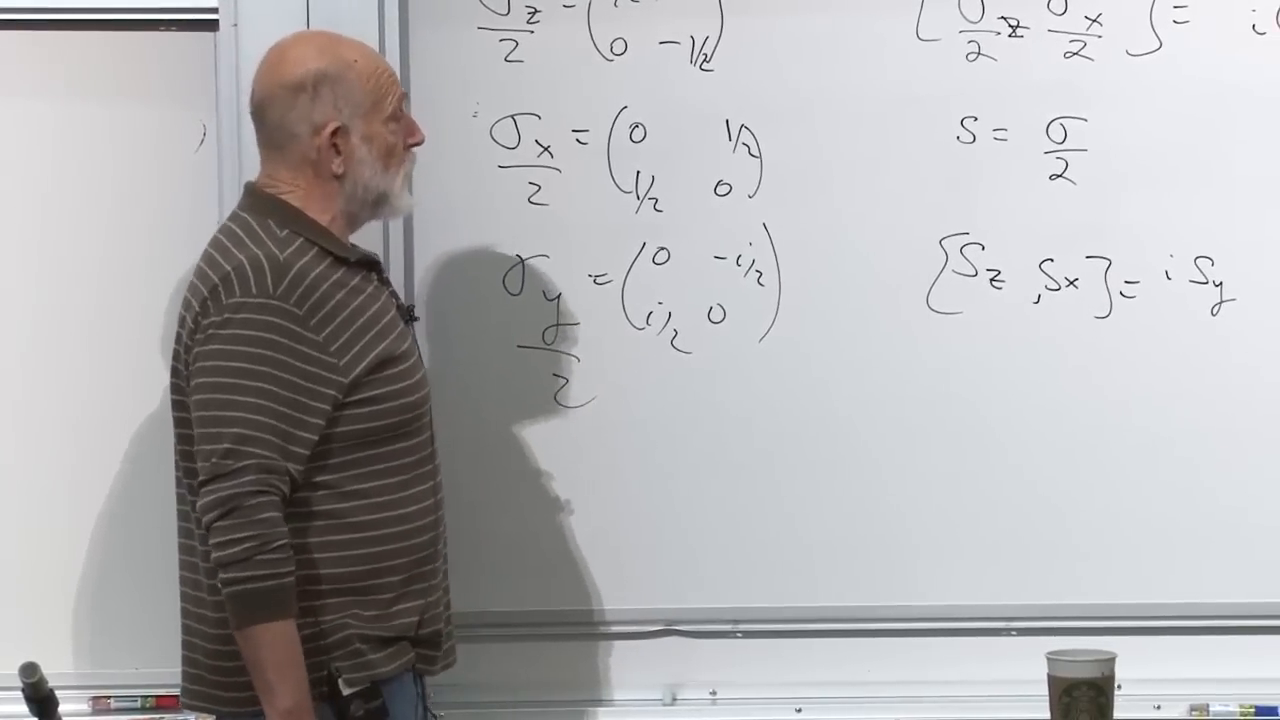
\includegraphics[width=0.9\linewidth]{lecture_04_frame_02.png}
\caption{В единицах, где \(\hbar=1\), половины матриц Паули являются операторами момента импульса для спина 1/2 и удовлетворяют соотношению \([S_z,S_x]=iS_y\).}
\lectureframe{00:55:41}
\end{figure}

Два уравнения на собственные значения для \(S_z\) имеют вид
\begin{equation}
S_z\lvert\pm\rangle
=\pm\frac{\hbar}{2}\lvert\pm\rangle.
\end{equation}
Эквивалентно, безразмерное магнитное квантовое число равно
\begin{equation}
m_{s}=\pm\frac12,
\qquad
S_{z}\lvert m_{s}\rangle
=m_{s}\hbar\,\lvert m_{s}\rangle.
\end{equation}
Операторы повышения и понижения момента импульса изменяют \(m\) целыми шагами, но это не требует, чтобы каждая лестница проходила через нуль. Целочисленные мультиплеты содержат целые значения \(m\), тогда как полуцелые мультиплеты содержат полуцелые значения. Для спина 1/2 лестница имеет только два члена \(m_s=+1/2\) и \(m_s=-1/2\).

Эти два состояния образуют дублет спина 1/2. К числу частиц, описываемых такими мультиплетами с полуцелым спином, относятся электроны, мюоны, нейтрино и кварки.

\section{Орбитальный и спиновый момент импульса}

Теперь имеются два вида момента импульса. Орбитальный момент импульса описывает движение относительно начала координат,
\begin{equation}
\mathbf L=\mathbf R\times\mathbf P,
\end{equation}
тогда как \(\mathbf S\) — внутренний спин. Их векторная сумма есть полный момент импульса,
\begin{equation}
\mathbf J=\mathbf L+\mathbf S.
\end{equation}

\begin{classroomqa}
\lecturetimestamp{00:56:49}
\audiencequestion{Если система имеет полный момент импульса \(\mathbf J\), как определить её спин \(\mathbf S\)?}
\lecturerresponse{Квантовые числа спина и орбитального момента обычно задаются отдельно. Если \(L=0\), весь момент импульса является спином. В противном случае нужны квантовые правила сложения моментов импульса, которые здесь пока откладываются.}
\end{classroomqa}

Правила сложения в равной мере применимы к сумме орбитального момента импульса и спина, к двум спинам или к двум орбитальным моментам импульса. Объединённая система имеет собственные допустимые значения полного момента импульса, но эти правила нам пока не нужны.

\begin{classroomqa}
\lecturetimestamp{00:58:18}
\audiencequestion{Какие экспериментальные данные привели к введению спина?}
\lecturerresponse{Свидетельства дала спектроскопия, но периодическая таблица даёт особенно наглядную мотивацию: её оболочечная структура требует, чтобы электроны обладали дополнительным двузначным свойством.}
\end{classroomqa}

\section{Водородоподобное вырождение и подсчёт оболочек}

Для орбитального момента импульса уравнение на собственные значения \(L^{2}\) имеет вид
\begin{equation}
L^{2}\lvert\ell,m\rangle
=\hbar^{2}\ell(\ell+1)\lvert\ell,m\rangle,
\end{equation}
и фиксированному значению \(\ell\) соответствуют
\begin{equation}
2\ell+1
\end{equation}
магнитных состояний, отвечающих \(m=-\ell,-\ell+1,\ldots,\ell\).

Идеальная нерелятивистская кулоновская задача имеет дополнительное вырождение. Энергии её связанных состояний отрицательны и стремятся к нулю снизу, но для подсчёта важно только выравнивание уровней. Первый уровень с \(\ell=1\) совпадает по энергии со следующим уровнем с \(\ell=0\); первый уровень с \(\ell=2\) присоединяется к следующей главной оболочке; и эта схема продолжается.\footnote{\texttt{lecture\_04\_frame\_03.png}, \(01{:}02{:}01\); полное выравнивание по главным оболочкам изложено с \(01{:}02{:}33\) по \(01{:}04{:}10\).}

\begin{figure}[htbp]
\centering
\begin{tikzpicture}[x=1.55cm,y=1.0cm]
\draw[->] (-0.65,0) -- (-0.65,4.35);
\draw[->] (-0.85,0) -- (4.75,0);
\node at (-0.95,4.08) {\(E\)};
\node at (4.55,-0.28) {\(\ell\)};
\node at (0,-0.30) {\(0\)};
\node at (2,-0.30) {\(1\)};
\node at (4,-0.30) {\(2\)};

\draw (-0.20,0.75) -- (0.20,0.75);

\draw (-0.20,2.00) -- (0.20,2.00);
\foreach \dx in {-0.18,0,0.18}
  \draw (2+\dx-0.06,2.00) -- (2+\dx+0.06,2.00);

\draw (-0.20,3.15) -- (0.20,3.15);
\foreach \dx in {-0.18,0,0.18}
  \draw (2+\dx-0.06,3.15) -- (2+\dx+0.06,3.15);
\foreach \dx in {-0.32,-0.16,0,0.16,0.32}
  \draw (4+\dx-0.05,3.15) -- (4+\dx+0.05,3.15);

\node[anchor=west] at (0.35,0.75) {\(n=1\)};
\node[anchor=west] at (2.35,2.00) {\(n=2\)};
\node[anchor=west] at (4.40,3.15) {\(n=3\)};
\end{tikzpicture}
\caption{Первые три идеальные кулоновские оболочки объединяют орбитальные мультиплеты с одинаковой главной энергией: одно состояние в первой оболочке, \(1+3\) во второй и \(1+3+5\) в третьей.}
\lectureframe{01:02:01}
\end{figure}

В главной оболочке \(n\) допустимые орбитальные квантовые числа таковы\footnote{Этот компактный диапазон \(\ell\) и приведённая ниже сумма воспроизводят выравнивание уровней и числа \(1,4,9,16,\ldots\), указанные с \(01{:}02{:}33\) по \(01{:}04{:}10\). Начало рисунка спектра показано в \texttt{lecture\_04\_frame\_03.png} при \(01{:}02{:}01\).}
\[
\ell=0,1,\ldots,n-1.
\]
Поэтому число пространственных состояний равно
\begin{equation}
\sum_{\ell=0}^{n-1}(2\ell+1)=n^{2},
\end{equation}
что даёт последовательность
\begin{equation}
1,\ 4,\ 9,\ 16,\ldots .
\end{equation}
Это только орбитальный подсчёт. Каждому пространственному состоянию соответствуют два значения спина, так что соответствующие идеализированные суммарные числа таковы
\begin{equation}
2,\ 8,\ 18,\ 32,\ldots=2n^{2}.
\end{equation}

\section{Принцип запрета и двузначное свойство электрона}

Начнём с гелия в приближении независимых электронов. Его ядро имеет заряд, вдвое больший протонного, что перескалирует водородоподобные уровни и стягивает электроны внутрь. Игнорируя пока электрон--электронные взаимодействия, два электрона могут занимать самую низкую пространственную орбиталь и давать разумное первое приближение к основному состоянию гелия.

Почему бы не поместить туда и третий электрон? Это понизило бы его орбитальную энергию, но так не происходит. Ограничение задаётся принципом запрета Паули: никакие два электрона не могут занимать одно и то же полное одночастичное состояние. Называть это обычной силой отталкивания было бы вводящим в заблуждение. Это ограничение на допустимое квантовое состояние.

Возникает кажущееся противоречие. Два электрона в гелии действительно занимают одну и ту же пространственную орбиталь. Разрешение состоит в том, что полное состояние электрона включает не только орбитальную волновую функцию. Оно также включает двузначную степень свободы. Назовём эти значения вверх и вниз. Один электрон на самой низкой орбитали может иметь спин вверх, а другой — спин вниз; их пространственные состояния совпадают, но полные квантовые состояния не совпадают.

На этом месте подсчёт сначала идёт вперёд к литию, а затем возвращается назад. Это возвращение показывает, почему необходимы и запрет, и спин. Представим себе правило запрета вообще без спина. Только один электрон мог бы занимать самое низкое пространственное состояние. Второй электрон должен был бы попасть в одно из четырёх пространственных состояний следующей главной оболочки, что дало бы несколько альтернатив там, где наблюдаемое основное состояние гелия единственно. Такая бесспиновая версия принципа запрета неверна.

Теперь восстановим два значения спина. Два электрона заполняют самую низкую орбиталь с противоположными спинами. Третий электрон, как в нейтральном литии, должен попасть в следующую главную оболочку. Эта оболочка имеет одно пространственное состояние \(\ell=0\) и три пространственных состояния \(\ell=1\). До учёта спина имеется четыре возможности.

\begin{classroomqa}
\lecturetimestamp{01:14:58}
\audiencequestion{Как состояния \(s\) и \(p\) дают 8 возможностей в первой возбуждённой оболочке?}
\lecturerresponse{Имеется одно пространственное состояние с \(\ell=0\) и три с \(\ell=1\), всего четыре пространственных состояния. Каждое допускает два значения спина, так что общее число равно \(2(1+3)=8\).}
\end{classroomqa}

Именно этот простой подсчёт лежит в основе восьми позиций во второй строке периодической таблицы. Это намеренная идеализация: из дальнейшего обсуждения станет ясно, что электрон--электронные взаимодействия вскоре нарушают картину независимых водородоподобных оболочек.

Это двузначное свойство можно также проверить, рассматривая его как угловой момент. Спин электрона сопровождается магнитным моментом, поэтому магнитное поле придаёт двум его спиновым проекциям разные энергии. Уровень, который был вырожден в отсутствие поля, расщепляется на два, как и следует ожидать для малого магнитного момента, направленного вдоль поля или против него. Это расщепление проверяет, ведёт ли добавленная двузначная степень свободы себя как угловой момент, а не как произвольная двоичная метка.

\section{Фотоны, электроны и пределы оболочечной модели}

Не все частицы подчиняются одному и тому же правилу заполнения состояний. Многие фотоны могут занимать одну и ту же электромагнитную моду; классическую световую волну можно понимать как состояние, содержащее большое число фотонов в этой моде. Электроны ведут себя иначе: принцип запрета не позволяет им скапливаться в одном и том же полном квантовом состоянии. Этот контраст и побуждает различать две статистики частиц.

\begin{classroomqa}
\lecturetimestamp{01:20:28}
\audiencequestion{Что происходит в случае свободного потока электронов, а не электронов, связанных в атомах?}
\lecturerresponse{Правило запрета по-прежнему действует: электроны не могут все занимать одно квантовое состояние. Лазер может поместить много фотонов в одну и ту же моду, но поток электронов нельзя подготовить таким образом.}
\end{classroomqa}

Это ограничение — свойство электронов, а не особенность связывания в атоме.

\begin{classroomqa}
\lecturetimestamp{01:21:12}
\audiencequestion{Орбитальный угловой момент — это именно вращение вокруг ядра?}
\lecturerresponse{Угловой момент определяется относительно выбранного начала отсчёта. В атоме естественным началом служит ядро, тогда как у свободной частицы относительно любого выбранного начала угловой момент равен \(\mathbf R\times\mathbf P\).}
\end{classroomqa}

Каждое обсуждение вращения предполагает выбор точки, относительно которой это вращение совершается. Атом задаёт естественный центр, потому что его ядро является центром приблизительно центрального потенциала. В свободном пространстве никакое начало не выделено, хотя угловой момент всё равно можно вычислить относительно любого выбранного начала.

\begin{classroomqa}
\lecturetimestamp{01:22:34}
\audiencequestion{Почему в периодической таблице повторяются сначала ряды по 8, а затем ряды по 18 элементов?}
\lecturerresponse{Простая оболочечная модель независимых электронов не объясняет полной картины. Она быстро перестаёт работать, потому что пренебрегает взаимодействиями между электронами.}
\end{classroomqa}

Для большого атома внешние электроны взаимодействуют со значительным внутренним электронным облаком, а также с ядром. Считать, что каждый электрон движется независимо в неэкранированном кулоновском поле, уже неразумно.

\begin{classroomqa}
\lecturetimestamp{01:23:33}
\audiencequestion{Почему атомы не становятся резко больше по мере добавления электронов?}
\lecturerresponse{Добавление электронов означает и добавление протонов в ядро. Возросший заряд ядра подтягивает внутренние электроны внутрь, а эти внутренние электроны экранируют ядро. В этой простой картине внешний валентный электрон тогда движется в поле эффективного заряда, примерно равного единице.}
\end{classroomqa}

Возросший ядерный заряд стягивает внутреннее облако. Для атома с одним внешним валентным электроном ядро и внутренние электроны на больших расстояниях почти компенсируют друг друга, оставляя валентный электрон в поле, приблизительно таком же, как поле единичного положительного заряда. Поэтому размеры атомов не растут просто пропорционально числу электронов.

\begin{classroomqa}
\lecturetimestamp{01:24:49}
\audiencequestion{Является ли электрическое отталкивание причиной того, что соседние атомы остаются разделёнными?}
\lecturerresponse{Само по себе — нет. Принцип запрета Паули даёт важное эффективное отталкивание при перекрытии электронных облаков, и для многих атомов именно оно является главной причиной того, что они сопротивляются дальнейшему перекрытию.}
\end{classroomqa}

Отталкивание Паули — это эффективное следствие запрета, а не отдельный закон взаимодействия.

\begin{classroomqa}
\lecturetimestamp{01:25:23}
\audiencequestion{Является ли принцип запрета отдельным постулатом?}
\lecturerresponse{В нерелятивистской квантовой механике он вводится как постулат. В релятивистской квантовой теории связь спин--статистика даёт ему более глубокое основание.}
\end{classroomqa}

\section{Тождественные частицы в классической и квантовой механике}

Прежде чем формулировать этот постулат, рассмотрим, как тождественные частицы подсчитываются в классической теории. Поместим две частицы одного и того же вида в набор ящиков. Если частицы втайне носят имена---Гарри и Салли---, то конфигурация, где Гарри в первом ящике, а Салли во втором, кажется отличной от конфигурации, где Салли в первом, а Гарри во втором.

Классическая механика допускает такую картину даже тогда, когда метки слишком слабы, чтобы их обнаружить. Можно вообразить на каждой частице сколь угодно слабую отметку и всё же считать их траектории различными. В классической статистической механике обычно предпочитают не считать перестановки тождественных частиц новыми конфигурациями. Для \(N\) частиц это соглашение даёт привычный множитель \(1/N!\).

Квантовая механика строже. Тождественные частицы не несут скрытых индивидуальных меток, которые в принципе можно было бы проследить. Два электрона взаимозаменяемы как электроны. Перестановка электрона с фотоном дала бы физически иное расположение, потому что это разные виды частиц, но перестановка двух электронных мест не может выявить, какой электрон в действительности был каким.

Одночастичному состоянию соответствует волновая функция
\[
\psi(x)=\langle x\vert\psi\rangle.
\]
Для двух частиц состояние является функцией двух координатных аргументов,
\begin{equation}
\psi(x_{1},x_{2}).
\end{equation}
Индексы обозначают два места в описании, а не два пространственных направления. Квадрат её модуля даёт совместную плотность вероятности положений.

\section{Оператор перестановки и постулат о статистике}

Поменяем местами два места, соответствующие частицам:
\begin{equation}
\psi(x_{1},x_{2})\longmapsto\psi(x_{2},x_{1}).
\end{equation}
Следуя обозначениям, используемым в этом обсуждении, обозначим оператор перестановки через \(S\). Здесь \(S\) обозначает обмен, а не вектор спина \(\mathbf S\). Он действует так:
\begin{equation}
(S\psi)(x_{1},x_{2})=\psi(x_{2},x_{1}).
\end{equation}
Произвольная функция двух переменных не обязана быть симметричной, так что эта операция может дать другую волновую функцию.

Двойная перестановка восстанавливает исходный порядок:
\begin{equation}
S^{2}=I.
\end{equation}
Перестановка обратима и сохраняет скалярные произведения, поэтому она представляется унитарным оператором. Если \(\psi\) — собственный вектор \(S\) с собственным значением \(\lambda\), то
\[
S^{2}\psi=\lambda^{2}\psi=\psi,
\]
и, следовательно,
\begin{equation}
\lambda=\pm1.
\end{equation}

Этот вывод выделяет два собственных подпространства оператора обмена, но он не утверждает, что всякая произвольная двухчастичная волновая функция уже является собственным вектором \(S\). Любую такую волновую функцию можно разложить на две части,\footnote{Это разложение представляет собой редакционное алгебраическое прояснение двух собственных подпространств, подразумеваемых \(S^{2}=I\). В записанном рассуждении сначала указываются два собственных значения, а затем вводится дополнительный статистический принцип.}
\begin{equation}
\psi_{\pm}=\frac12(I\pm S)\psi,
\end{equation}
которые удовлетворяют
\begin{equation}
S\psi_{\pm}=\pm\psi_{\pm}.
\end{equation}
Следовательно,
\begin{align}
\psi_{+}(x_{2},x_{1})&=\psi_{+}(x_{1},x_{2}),\\
\psi_{-}(x_{2},x_{1})&=-\psi_{-}(x_{1},x_{2}).
\end{align}

Теперь вводится дополнительный принцип, не являющийся следствием одного лишь \(S^{2}=I\). Для тождественных частиц любого фиксированного вида допустимые состояния целиком лежат в одном из этих секторов обмена: перестановка пары либо всегда оставляет ту же волновую функцию, либо всегда меняет её знак. Сектор \(+1\) симметричен, а сектор \(-1\) антисимметричен. Физическая интерпретация этих двух возможностей как двух статистик частиц — следующий шаг, и он оставлен для последующего обсуждения.
